\chapter{Gewöhnliche Differenzialgleichungen}
Eine Gleichung, in der Ableitungen einer gesuchte Funktionen auftreten, nennt man Differentialgleichung.
$$y'(t)=y+y^2$$
$$\left( y'(t)\right)^2=y(t)+2$$
Hängt die gesuchte Funktion in der DGL nur von einer einzigen variablen ab, so spricht man von einer ''gewöhnliche DGL''.\\

\noindent Hängt hingegen die gesuchte Funktion von mehrere Variabeln ab, d.h. kommen partielle Ableitungen in der Differentialgleichung vor, so liegt eine ''Partielle DGL'' vor. Viele physikalische Prozesse lassen sich oft durch Differenzialgleichungen bescreiben.
\subsubsection*{Besipiel}
\begin{enumerate}
\item Ein lineares Federpendel wird durch folgende DGL beschrieben $$m\frac{d^2x}{dt^2}=-Kx\text{\hspace{10mm} mit K = Federkonstante}$$
\begin{center}
\begin{tikzpicture}
\node[circle,fill=black,inner sep=1.5mm] (a) at (0,0) {};
\draw[decoration={aspect=0.3, segment length=2mm, amplitude=2mm,coil},decorate] (2,0) -- (0.5,0); 
\draw[decoration={aspect=0.3, segment length=2mm, amplitude=2mm,coil},decorate] (-2,0) -- (-0.5,0); 
\draw (0.5,0)--(0,0);
\draw (-0.5,0)--(0,0);
\draw (2,0)--(2.5,0);
\draw (-2,0)--(-2.5,0);

\fill [pattern = north east lines] (-2.5,-0.5) rectangle (-2.7,0.5);
\draw[thick] (-2.5,0.5) -- (-2.5,-0.5);
\fill [pattern = north east lines] (2.5,-0.5) rectangle (2.7,0.5);
\draw[thick] (2.5,0.5) -- (2.5,-0.5);

\draw[] (0,-0.8) -- (0,-0.3);
\draw[->] (0,-0.55) -- (1,-0.55);
\node[] at (1.5,-0.55){$x(t)$};
\end{tikzpicture}
\end{center}
Unbekannt ist hier die Auslenkung $x$ in Abhängigkeit von der Zeit $t$
\item Beim radioaktiven Zerfall, haben wir $$\frac{df(t)}{dt}=-\alpha f\text{\hspace{10mm}}f(0)=f_0$$
wobei $f(t)=$ die noch vorhandeden Masse eines Stoffes. Pro zeiteinheit zerfallende Masse ist proportional zur noch vorhandene Masse
\item Freier Fall mit Reibung
\begin{center}
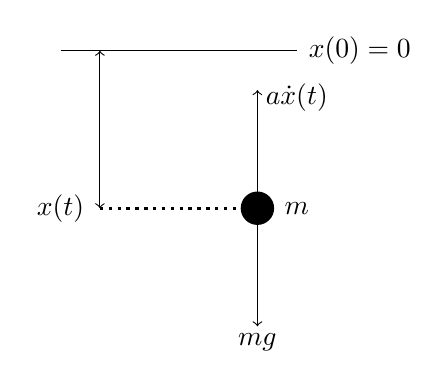
\begin{tikzpicture}
\node[circle,fill=black,inner sep=1.5mm] (a) at (0,0) {};
\draw[<->](-2,0)--(-2,2);
\draw[->] (0,0) -- (0,1.5);
\draw[->] (0,0) -- (0,-1.5);
\draw[] (-2.5,2) -- (0.5,2);
\draw[dotted, very thick] (-2,0) -- (0,0);
\node[] at (-2.5,0){$x(t)$};
\node[] at (1.3,2){$x(0)=0$};
\node[] at (0.5,0){$m$};
\node[] at (0.5,1.4){$a\dot x(t)$};
\node[] at (0,-1.7){$mg$};
\end{tikzpicture}
\end{center}
Sei $m$ eine Massepunkt der Unter Einfluss der Schwerkraft fällt. Es kann auch ein Reibungskraft geben. \\

Die grösse der Reibungskraft ist proportional zur Geschwindigkeit. Dann ist, nach der zweiten Newtonische Gesetzt \[m\ddot x = mg - a\dot x\text{\hspace{10mm}}v=\frac{dx}{dt}\]
Beim 2., haben wir schon letze Semester gesehen dass $$\frac{df(t)}{dt}=-\alpha f$$ als eine Lösung $Ke^{-\alpha t}$, $K\in\mathbb{R}$
$$f'=-\alpha t\Rightarrow \frac{f'}{f}=-\alpha$$
$$\int{\frac{f'(t)}{f(t)}dt}=-\int{\alpha dt}$$
$$\ln\left| f(t)\right|=-\alpha t+C$$
$$\Rightarrow f(t)=Ke^{-\alpha t}\text{ mit }K={e^{t}}^C$$
\end{enumerate}
Alle 3 Beispiele sind Lineare DGL mit konstanten Koeffizienten. 
\section{Lineare DGL mit konstante Koeffizienten} 
\begin{framed}
\centerline{\textbf{Definition 7.1}}
\noindent Eine lineare Differentialgleichung $n-$ter Ordnung hat die Gestalt \[{y^{(n)}} + {a_{n - 1}}(x){y^{(n - 1)}} +  \ldots  + {a_1}(x)y' + {a_0}(x)y = b(x)\] mit $a_i(x),i=0,\dots,n-1, b(x)$ Funktionen. 
\end{framed} \todo{Where is the end of the definition??}
Ist das so genannte Störfunktion $b(x)$ konstant gleich 0, so heisst die DGL homogen, andernfalls inhomogen. Im Falle $a_i(x)=a_i$ Konstanten, heisst die LDG, LDG mit Konstanten koeffizioenten. \\

In diesem Abschnitt betrachten wir DGL mit konstanten Koeffizienten. Eine DGL ist genau dann linear wenn alle Potenzen der gesuchte Funktion und deren Ableitung(en) nur mit Potenz 1 vorkommen.
z.B.:
\begin{itemize}
\item $\left( y'\right)^2+y^2=1$ ist nicht linear
\item $y'=2xy$ ist linear
\item $y'=\sqrt{y}+1$ ist nicht linear
\item $y''+2y'+x=0$ ist linear
\end{itemize}

\noindent Zum nächst betrachten wir Homogene LDG mit konstanten Koeffizienten. Sei $$y^{(n)}+a_{n-1}y^{(n-1)}+\dots+a_0=0\text{\hspace{10mm}(H)}$$ wobei $a_i\in\mathbb{R}$ $i=0,\dots,n-1$
\begin{framed}
\centerline{\textbf{Definition 7.2}}
\noindent Das charakteristische Polynom der Gleichung (H) ist gegeben durch $$p(t):=t^n+a_{n-1}t^{n-1}+\dots+a_0$$
\end{framed} 
\subsubsection*{Lemma 7.3}
Die Funktion $y(x)=e^{\lambda x}$ ist genau dann Lösung von (H) falls $p(\lambda)=0$ 
\subsubsection*{Beweis}
$$y(x)=e^{\lambda x}$$
$$y'(x)=\lambda e^{\lambda x}$$
$$y^j(x)=\lambda ^je^{\lambda x}$$
Also mit $$=y^{(n)}(x)+a_{n-1}y^{(n-1)}(x)+\dots+a_0=(\lambda ^n+a_{n-1}\lambda ^{n-1}+\dots +a_0)e^x=$$
$$\Leftrightarrow \lambda^n+a_{n-1}\lambda^{n-1}+\dots +a_0=p(\lambda)=0$$

\subsubsection*{Satz 7.4}
Sei $p(\lambda ) = \prod\limits_{i = 1}^l {{{(\lambda  - {\lambda _i})}^{{m_i}}}} $ mit $\lambda _j\in\mathbb{C}$, $\lambda_i\not=\lambda_j (i\not=j)$. Dann ist jede Lösung der zugehörigen HDGL darstellbar als Linearkombination der $n$ linear unabhängigen Funktionen $y_{ik}(x)=x^ke^{\lambda_ix}$, \todo{Can't understand limits, page 81 bottom}

\subsubsection*{Bemerkung 7.5}
\begin{enumerate}
\item Falls die characteristischen Polynom $n$ verschiedene reelle Nullstelle $\lambda_1,\dots,\lambda_n$ besitzt, so bilden ${e^{{\lambda _1}x}},{e^{{\lambda _2}x}}, \ldots ,{e^{{\lambda _n}x}}$ eine Basis des Vektorraums der Lösungen, das heisst für jede Lösung $y(x)$gibt es $c_1,c_2,\dots,c_n$ so dass $$y(x)={c_1}{e^{{\lambda _1}x}} + {c_2}{e^{{\lambda _2}x}} +  \ldots  + {c_n}{e^{{\lambda _n}x}}$$

\item Sei $\lambda$ eine $k-$fache reelle Nullstelle das charakteristisches polynoms. Dann sind $$e^{\lambda x},xe^{\lambda x},\dots ,x^{k-1}e^{\lambda x}$$ $k$ linear unabhängige Lösungen. 
\item Sind $\lambda=\alpha+i\beta$, $\overline{\lambda}=\alpha-i\beta$, \todo{What ?? page 82 bottom} ein Paar konjugiert komplexer $k-$ fache nullstellen, so sind die Funktionen\\\begin{center}
\begin{tabular}{c c c}
$e^{\alpha x}\cos\left(\beta x\right)$&\hspace{10mm}&$e^{\alpha x}\sin\left(\beta x\right)$\\
\vdots&\hspace{10mm} & \vdots\\
$x^{k-1}e^{\alpha x}\cos\left(\beta x\right)$&\hspace{10mm}&$x^{k-1}e^{\alpha x}\sin\left(\beta x\right)$\\
\end{tabular}
\end{center}
2$k$ linear unabhängige Lösungen der DGL \[\left( {{e^{\left( {\alpha  + i\beta } \right)x}} = {e^{\alpha x}} \cdot {e^{i\beta x}} = {e^{\alpha x}}\cos \left( {\beta x} \right) + i{e^{\alpha x}}\sin \left( {\beta x} \right)} \right)\]
\end{enumerate}

\subsubsection*{Besipiel 7.6}
\begin{enumerate}
\item $$y''-y=0$$
$$p(\lambda)=\lambda^2-1=0=(\lambda-1)(\lambda+1)$$
$$y(x)=c_1e^x+c_2e^{-x}$$
\item $$y''+y=0$$
$$p(\lambda)=\lambda^2+1=(\lambda+1)(\lambda-1)$$
$$y(x)=c_1\cos x+c_2\sin x$$
\item $$y^{(4)}+2y^{(2)}+y=0$$
$$p(\lambda)=\lambda^4+2\lambda^2+1=0=(\lambda^2+1)^2=(\lambda-i)^2(\lambda+i)^2$$
Also, $\cos x, \sin x, x\cos x,x\sin x$ sind Lösungen. \todo{is there  subscript like $y_1(x)$?? page 84 middle}$$y(x)=c_1\cos x+c_2 x\cos x+c_3\sin x+c_4 x\sin x$$
\item $$y^{(4)}-y=0$$
$$p(\lambda)=t^4-1=(t^2-1)(t^2+1)=(t+1)(t-1)(t+i)(t-i)$$
$$y(x)=c_1e^x+c_2e^{-x}+c_3\sin x+c_4\cos x$$
\item $$2y''+20y'+48y=0$$
$$p(\lambda)=2\lambda^2 +20\lambda+48=0\Rightarrow \lambda_{1,2}=-4,-6$$ 
Die Lösung ist $$y(x)=c_1e^{-4x}+c_2e^{-6x}$$
\end{enumerate}
\section{Inhomogene DGL}
Bisher haben wir nur Homogene Lineare DGL mit konstanten Koeffizienten betrachtet. Sehr oft treten auch Zusatzterme in den Gleichung auf. Wir haben der Folgende Allgemeine Satz für die Lösungsstruktur linearer DGL
\subsubsection*{Satz 7.7}
Die allgemeine Lösung einer inhomogenen DGL $$y^{(n)}+a_{n-1}y^{(n-1)}+\dots +a_1y'+a_0y=b(x)$$ ist die Summe einer ''spezielle'' Lösung der inhomogenen DGL und der allgemeinen Lösung der zugehörigen homogenen DGL $$\underbrace {{y_A}(x)}_{\scriptstyle{\text{Allgemeine Losung }}\hfill\atop
\scriptstyle{\text{der inhomogene DGL}}\hfill} = \underbrace {{y_S}(x)}_{\scriptstyle{\text{Spezielle Losung }}\hfill\atop
\scriptstyle{\text{der inhomogene DGL}}\hfill} + \underbrace {{y_{AH}}(x)}_{\scriptstyle{\text{Allgemeine Losung }}\hfill\atop
\scriptstyle{\text{der Homogene DGL}}\hfill}$$
\subsubsection*{Besipiel}
$$y''+y=\sin x$$
Um diese inhomogene DGL zu lösen, benötigen wir die allgemeine Lösung der zugehörigen homogene DGL $y''+y=0$$$p(\lambda)=\lambda^2+1=0\Rightarrow y_{AH}(x)=c_1\sin x+c_2\cos x$$ Nun wird noch eine spezielle Lösung der inhomogene DGL $y''+y=\sin x$ benötigt. Wir verifizieren dass $y(x)=-\frac{1}{2}x\cos x$ eine derartige Lösung ist
$$y'(x)=-\frac{1}{2}\cos x+\frac{1}{2}x\sin x$$
$$y''(x)=\frac{1}{2}\sin x+\frac{1}{2}\sin x+\frac{1}{2}x\cos x=\sin x+\frac{1}{2}x\cos x$$
$$y''(x)+y(x)=\sin x+\frac{1}{2}x\cos x-\frac{1}{2}x\cos x=\sin x$$ Die allgemeine Lösung der inhomogenes DGL ist damit $$y(x) = \underbrace { - \frac{1}{2}x\cos x}_{\scriptstyle{\text{Spezielle Losung }}\hfill\atop
\scriptstyle{\text{der inhomogene DGL}}\hfill} + \underbrace {{c_1}\sin x + {c_2}\cos x}_{\scriptstyle{\text{Allgemeine Losung }}\hfill\atop
\scriptstyle{\text{der Homogene DGL}}\hfill}$$
\subsubsection*{Bemerkung}
Man kann als Speziell Lösung der inhomogenes DGL auch $$y(x)=-\frac{1}{2}x\cos x+5\sin x$$ wählen. Dann gilt auch hier $y''+y=\sin x$. Die allgemeine Lösung der inhomogenes DGL 
$$y(x) = \underbrace { - \frac{1}{2}x\cos x + 5\sin x}_{\scriptstyle{\text{Spezielle Lösung }}\hfill\atop
\scriptstyle{\text{inhomogenes DGL}}\hfill} + \underbrace {{k_1}\sin x + {k_2}\cos x}_{\scriptstyle{\text{Allgemeine Lösung }}\hfill\atop
\scriptstyle{\text{homogenes DGL}}\hfill}$$ Sie unterscheidet sich nicht von der Lösung $$y(x)=-\frac{1}{2}x\cos x+c_1\sin x+c_2\cos x$$$$c_1=5+k$$
\subsubsection*{Frage:}
Wie kann man eine spezielle Lösung finden?
\subsubsection*{Antwort:}
Zur Lösung der inhomogenes DGL kann man in vielen Fällen einen so genannte ''Ansatz vom Typ der rechten Seite'' wählen. Hier geht man davon aus, dass die Lösung die gleiche Gestalt wie die Störfunktion haben wird.\\

\noindent z.B.: ist die Störfunktion ein Polynom, so nimmt man an, dass die spezielle Lösung auch ein polynom sein wird. Ist die Störfunktion ein exponentialfunktion so nimmt man an, dass die Lösung auch ein exponentialfunktion sein wird.

\subsubsection*{Besipiel 7.8}
\begin{enumerate}
\item Wir betrachten die DGL $$y''+y'-6y=3e^{-4x}$$Die Zugehörige homogenes DGL $$y''+y'-6y=0$$$$p(\lambda)=\lambda^2+\lambda-6=0\text{\hspace{5mm}}\lambda_{1,2}=2,-3$$ Die Allgemeine Lösung der Homogenes DGL ist $$y(x)=c_1e^{-3x}+c_2e^{2x}$$ Zur Lösung der inhomogenes DGL verwenden wir einen ''Ansatz vom Typ der Rechten Seite'', gehen also davon aus, dass die spezielle Lösung der inhomogenes DGL die ähnliche Gestalt hat (als die Störfunktion) $$y_s(x)=Ke^{-4x}$$Für die Ableitungen des Ansatzes haben wir $$y_s'(x)=-4Ke^{-4x}$$$$y''_s(x)=16Ke^{-4x}$$Eingesetzt in die homogenes DGL ergibt sich $$y''+y'-6y=16Ke^{-4x}-4Ke^{-4x}-6Ke^{-4x}=6Ke^{-4x}=3e^{-4x}$$Also $6K=3\Rightarrow K=\frac{1}{2}$. Damit ist $y_s(x)=\frac{1}{2}e^{-4x}$ und die allgemeine Lösung der DGL $$y(x)=\frac{1}{2}e^{-4x}+c_1e^{-3x}+c_2e^{2x}\text{\hspace{5mm}}c_1,c_2\in\mathbb{R}$$
\item $$y''+y'-6y=50\sin x$$ Wählen wir als ''Ansatz vom Typ der rechten Seite''

$${y_s}(x) = {K_1}\sin x + {K_2}\cos x$$
$$y{'_s}(x) = {K_1}\cos x - {K_2}\sin x$$
$$y'{'_s}(x) =  - {K_1}\sin x - {K_2}\cos x$$
$$y'' + y' - 6y =  - {K_1}\sin x - {K_2}\cos x + {K_1}\cos x - {K_2}\sin x + 6{K_1}\sin x + 6{K_2}\cos x$$
$$ = ( - 7{K_1} - {K_2})\sin x + ( - 7{K_2} + {K_1})\cos x$$
$$ = 50\sin x$$
$$ \Rightarrow  - 7{K_2} + {K_1} = 0 \Rightarrow {K_1} = 7{K_2}$$
$$ - 7{K_1} - {K_2} = 50 \Rightarrow  - 49{K_2} - {K_2} = 50$$
$$ \Rightarrow {K_2} =  - 1,{K_1} =  - 7$$
$$y_s(x)=-7\sin x-\cos x$$
Damit ist die allgemeine Lösung der inhomogenes DGL $$y(x)=-7\sin x-\cos x+c_1e^{-3x}+c_2e^{2x}$$
\end{enumerate}
Ein problem ergibt sich, wenn als Störfunktion eine Lösung der homogenes DGL erscheint:
\begin{enumerate}[\indent 3.]
\item $$y''+y'-6y=e^{2x}$$''Der Ansatz vom Typ der rechten Seite''$$y(x)=Ke^{2x}$$ führt nicht weiter da dieser Ansatz eingesetzt in homogenes DGL 0 ergeben muss und nicht $e^{2x}$. Wir führen nun der Ansatz
$$y(x)=Kxe^{2x}$$
$$y'(x) = K{e^{2x}} + 2Kx{e^{2x}}$$
$$y''(x) = 2K{e^{2x}} + 2K{e^{2x}} + 4Kx{e^{2x}}$$
$$y'' + y' - 6y = 4Kx{e^{2x}} + 4Kx{e^{2x}} + K{e^{2x}} + 2Kx{e^{2x}} - 6Kx{e^{2x}}$$
$$ = 5K{e^{2x}} = 10{e^{2x}}$$
$$\Rightarrow K=2$$
Der Ansatz führte also auf die Lösung $$y_s(x)=2xe^{2x}$$
Ingesamt: $$y(x)=2xe^{2x}+c_1e^{-3x}+c_2e^{2x}\text{\hspace{5mm}}c_1,c_2\in\mathbb{R}$$
\item $$y''+y=\sin x$$$$y_H=c_1\sin x+c_2\cos x$$
Für die Spezielle Lösung zu finden, wählen wir den Ansatz vom Typ der rechten Seite
$${y_s}(x) = x\left( {{K_1}\sin x + {K_2}\cos x} \right)$$
$$y{'_s}(x) = \left( {{K_1}\sin x + {K_2}\cos x} \right) + x\left( {{K_1}\cos x - {K_2}\sin x} \right)$$
$$y'{'_s}(x) = {K_1}\cos x - {K_2}\sin x + {K_1}\cos x - {K_2}\sin x + x\left( { - {K_1}\sin x - {K_2}\cos x} \right)$$
Eingesetzt in die DGL ergibt sich
$$y'{'_s}(x) + y(x) = 2{K_1}\cos x - 2{K_2} - x({K_1}\sin x + {K_2}\cos x) + x({K_1}\sin x + {K_2}\cos x)$$
$$=2K_1\cos x-2K_2 \sin x=\sin x$$
$$\Rightarrow 2K_1=0, -2K_2=1\Rightarrow K_1=-\frac{1}{2}$$
$$\Rightarrow y_s(x)=-\frac{1}{2}x\cos x$$
$$y_A=-\frac{1}{2}x\cos x+c_1 \sin x+c_2\cos x$$
\end{enumerate}
